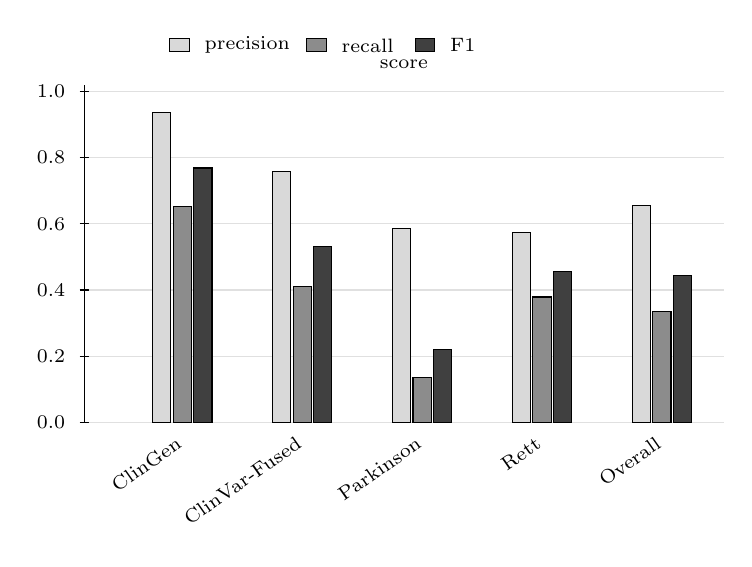
\begin{tikzpicture}[
  font=\scriptsize,
  x=1.45cm,
  y=4.2cm,
  axis/.style={black, thin},
  tick/.style={black, thin},
  precision/.style={fill=black!15, draw=black},
  recall/.style={fill=black!45, draw=black},
  fone/.style={fill=black!75, draw=black},
]
  \draw[axis] (-0.6,0) -- (5.0,0);
  \draw[axis] (-0.6,0) -- (-0.6,1.02);

  \foreach \y/\label in {0/0.0,0.2/0.2,0.4/0.4,0.6/0.6,0.8/0.8,1.0/1.0} {
    \draw[tick] (-0.64,\y) -- (-0.56,\y);
    \node[anchor=east] at (-0.68,\y) {\label};
    \draw[black!12] (-0.56,\y) -- (5.0,\y);
  }

  % ClinGen
  \draw[precision] (0.00,0) rectangle (0.16,0.938);
  \draw[recall] (0.18,0) rectangle (0.34,0.652);
  \draw[fone] (0.36,0) rectangle (0.52,0.769);
  \node[anchor=east, rotate=35] at (0.30,-0.04) {ClinGen};

  % ClinVar-Fused
  \draw[precision] (1.05,0) rectangle (1.21,0.758);
  \draw[recall] (1.23,0) rectangle (1.39,0.410);
  \draw[fone] (1.41,0) rectangle (1.57,0.532);
  \node[anchor=east, rotate=35] at (1.35,-0.04) {ClinVar-Fused};

  % Parkinson
  \draw[precision] (2.10,0) rectangle (2.26,0.587);
  \draw[recall] (2.28,0) rectangle (2.44,0.136);
  \draw[fone] (2.46,0) rectangle (2.62,0.221);
  \node[anchor=east, rotate=35] at (2.40,-0.04) {Parkinson};

  % Rett
  \draw[precision] (3.15,0) rectangle (3.31,0.574);
  \draw[recall] (3.33,0) rectangle (3.49,0.379);
  \draw[fone] (3.51,0) rectangle (3.67,0.456);
  \node[anchor=east, rotate=35] at (3.45,-0.04) {Rett};

  % Overall
  \draw[precision] (4.20,0) rectangle (4.36,0.655);
  \draw[recall] (4.38,0) rectangle (4.54,0.336);
  \draw[fone] (4.56,0) rectangle (4.72,0.444);
  \node[anchor=east, rotate=35] at (4.50,-0.04) {Overall};

  \node[anchor=south] at (2.20,1.04) {score};

  \draw[precision] (0.15,1.12) rectangle (0.32,1.16);
  \node[anchor=west] at (0.37,1.14) {precision};
  \draw[recall] (1.35,1.12) rectangle (1.52,1.16);
  \node[anchor=west] at (1.57,1.14) {recall};
  \draw[fone] (2.30,1.12) rectangle (2.47,1.16);
  \node[anchor=west] at (2.52,1.14) {F1};
\end{tikzpicture}
